\subsection[Non-isothermal single-phase flow]{Non-isothermal single-phase flow of different fluids with variable fluid properties (HT-process)}
\label{eos-ht-example}

\subsubsection*{Problem definition}

The aim of this test case is to show the functionality of different equations of state and transport property correlations for different fluids. Because of that, the model setup from section \ref{eos-h-example} was extended by non-isothermal conditions. At the beginning of the infiltration, the residing fluid within the reservoir has a temperature of $\unit[400]{K}$. At the point of injection, a constant temperature of $\unit[300]{K}$ is defined. During the infiltration process, the reservoir will cool down and the residing fluid will change its properties. In case of \co2 as working fluid, there will be a phase change during the injection process regarding the \co2 phase diagram in Fig.~\ref{fig-eos-phase}. Note that this example shows just the fluid behavior related to temperature and pressure conditions. No physically based phase change is simulated here, only the fluid property functions are tested.\\[1.5ex] 

This example is simulated for four different substances (\co2, \ch4, \h2o, and \n2). For each substance, three different EOS are tested, so that this test case consists of twelve model set ups. Tab.~\ref{tab-eos-fluid_prop_bm} gives an overview about the used fluid property correlations.

\begin{figure}[h]
\centering
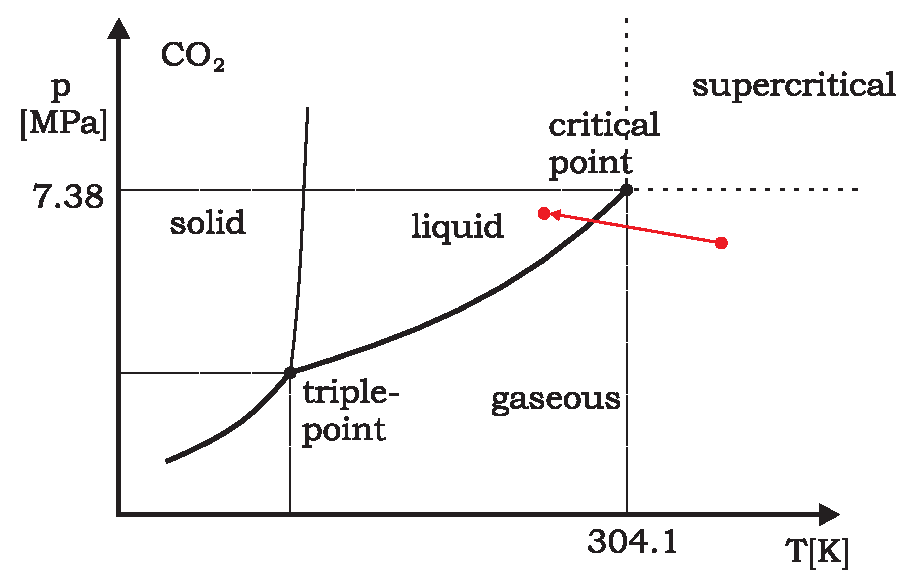
\includegraphics[width=0.8\textwidth]{FLUID_PROPERTIES/figures/phase-diagram-co2.eps}
\caption{Phase diagram of carbon dioxide. The two extreme conditions ($\unit[400]{K}$ at $\unit[6.5]{MPa}$ and $\unit[300]{K}$ at $\unit[7]{MPa}$) are crossing a phase boundary of \co2, so a phase change from hot gas to  to liquid state will be forced.}
\label{fig-eos-phase}
\end{figure}

%
\begin{table}[htbp]
\caption{Set-up names and referring correlation functions}
%\centering
\label{tab-eos-fluid_prop_bm}
\begin{center} 	
\begin{tabular}{llll}
\toprule
\textbf{working fluid} 	& \textbf{model name}   & \textbf{density} 	& \textbf{viscosity}  \\
\midrule
Methane \ch4			& CH4-RK     			&  \cite{RedKwo:49} & Friend, 1989 \cite{FriElyIng:89}\\
            			& CH4-PR     			&  \cite{PenRob:75} &    \\
             			& CH4-HE    			&  \cite{SetWag:91} &    \\
\midrule
Carbon dioxide \co2 	& CO2-RK     			&  \cite{RedKwo:49}  & Fenghour, 1998 \cite{FenWakVes:98} \\
                    	& CO2-PR     			&  \cite{PenRob:75}  &    \\
                   		& CO2-HE     			&  \cite{SpaWag:96}  &    \\
\midrule
Water \h2o 				& H2O-RK     			&  \cite{RedKwo:49}  & IAPWS, 1998 \cite{IAPWS:08a}      \\ 
           				& H2O-PR     			&  \cite{PenRob:75}  &    \\
           				& H2O-HE     			&  \cite{WagPru:02}  &    \\
\midrule
Nitrogen \n2 			& N2-RK      			& \cite{RedKwo:49}   & Stephan, 1987 \cite{SteKraLae:87} \\
             			& N2-PR     			&  \cite{PenRob:75}  &    \\
             			& N2-HE     			&  \cite{SpaLem:00}  &    \\
\bottomrule
\end{tabular}
\end{center}
\end{table}


\subsubsection*{Model setup}

The 1D model domain of this test case consists of 200 line elements with a length of $\unit[0.5]{m}$. There is an injection well on the left, and a production well on the right side (see Fig.~\ref{fig-eos-ms-bt2}). The thermal properties of the porous medium was all set to zero, so that no heat is stored or transported by the solid material. The fluid pressure on the left hand side (injection point) is $\mathrm{p}=\unit[7]{MPa}$, on the right hand side the pressure is $\mathrm{p}=\unit[6.5]{MPa}$. Tab.~\ref{eos-co2-flow-mod-spec} gives an overview about the model specifications.

\begin{figure}[ht]
\centering
\includegraphics[width=0.7\textwidth]{FLUID_PROPERTIES/figures/Modelsetup-nlgwft.eps}
\caption{Model setup}
\label{fig-eos-ms-bt2}
\end{figure}


\begin{table}%[ht]
\caption{HT-benchmark specifications}
%\centering
\label{eos-co2-flow-mod-spec} 
\begin{center}
\begin{tabular}{lrr}
\toprule
\textbf{parameter}   			& \textbf{symbol} 	& \textbf{value} \\
\midrule
\textit{spatial discretisation} &  					&  \\
model dimension:     			&	            	& 1D               \\
no. of Elements:    			&              		& 200              \\
length :             			& L            		& \unit[100]{m} \\ 
step size:           			& $\delta x$   		& \unit[0.5]{m} \\
\midrule
\textit{initial conditions} 	& 					& \\
temperature:         			& T            		& \unit[400]{K} \\
pressure:            			& p            		& \unit[6.5]{MPa} \\
\midrule
\textit{boundary conditions} 	& 					& \\
pressure (left):     			& p            		& \unit[7.0]{MPa} \\
pressure (right):    			& p            		& \unit[6.5]{MPa} \\
temperature (left):  			& T            		& \unit[300]{K} \\
\midrule
\textit{temporal discretisation} & 					& \\
timesteps:           			& $\Delta t$   		& \unit[$10\,000$]{s}  \\ 
no. of timesteps:    			&              		& 30    \\
total time:          			&     t        		& \unit[$30\,000$]{s}  \\

\midrule

\textit{fluid properties}    	& 					& \\
density:             			& $\rho$       		& \small{simulated}  \\
viscosity:           			& $\eta$       		& \small{simulated}  \\
heat capacity        			& $c$          		& \unit[40]{W$\cdot$m$^{\text{-1}}\cdot$K$^{\text{-1}}$} \\
heat conductivity    			& $\lambda$    		& \unit[0.06]{J$\cdot$m$^{\text{-}1}\cdot$K$^{\text{-}1}$} \\
\midrule
\textit{reservoir properties} 	& 					& \\
thermal conductivity 			& $\lambda$    		& - \\
heat capacity:       			& $c$         		& - \\
density:             			& $\rho$       		& - \\
\bottomrule
\end{tabular}
\end{center}
\end{table}

\subsubsection*{Results}

Fig.~\ref{fig-eos-bt2} shows the distribution of the fluid density and its viscosity after a simulation time of 50\,000 seconds. At this time, the phase border has moved $\unit[175]{m}$ away from the injection well. At this point, the density jumps from $\unit[475]{kg\cdot m^{-3}}$ down to $\unit[220]{kg\cdot m^{-3}}$. The stepwise droping of density between $\unit[175]{m}$ and $\unit[300]{m}$ is caused by the interpolation of database values. A higher resolution of density values in the database should solve this problem. The "saw teeth" and the offset between $\unit[60]{m}$ and $\unit[120]{m}$ is also caused by the interpolation, but this time the problem is deeper. Here, the interpolation takes place between liqiud ant gaseous density values. To solve this problem, the FCT-reading function has to be enhanced by a switch which avoids a interphase interpolation.

\begin{figure}[ht]
\centering
\includegraphics[width=0.8\textwidth]{FLUID_PROPERTIES/figures/CO2-EOS-HT.eps}
\caption{This is still a dummy graphic, the correct result plot follows soon...}
\label{fig-eos-bt2}
\end{figure}
